\section{Legacy: Who Won and What Remains}

\subsection{End of Apollo and later cooperation}
After Apollo 11, the United States flew several more lunar missions before ending the program in 1972, as budgets tightened and priorities shifted. The Soviet crewed lunar effort, hampered by the failures of its giant N1 rocket and the death of Korolev, never reached the Moon at all.

The N1 told the Soviet half of the ending. Four launches between 1969 and 1972 ended in four failures, including an explosion that destroyed its pad, and the program was cancelled in secrecy so complete that Moscow denied for years that a crewed lunar effort had existed. The cover story held until the archives opened decades later.

Competition gradually gave way to contact. In 1975 the Apollo-Soyuz Test Project docked American and Soviet spacecraft in orbit, a symbolic handshake that signaled the race's most intense phase was over.

The handshake required real engineering diplomacy. The two nations designed a shared docking adapter, reconciled incompatible atmospheres and procedures, and trained crews in each other's languages and simulators. The techniques of working together, negotiated by the same establishments that had raced each other, outlasted the mission.

Both programs redirected their remaining hardware toward orbital stations. The Soviet Union flew the Salyut series and learned long-duration spaceflight the hard way, while the United States converted a Saturn stage into Skylab and kept three crews aloft for months. The race's leftover machines, built to reach the Moon, ended up teaching both nations how to live in orbit instead.

The last three planned Apollo missions were cancelled with their Saturn rockets already built, and the giant vehicles became museum pieces in Houston, Huntsville, and Florida. Ending the program while the hardware still worked struck many engineers as a waste; to the budget committees it was simply what victory looked like once the race had been won.

That thaw set a precedent. The cooperation rehearsed in the 1970s would later mature into joint programs, culminating in the International Space Station, where former rivals share a single laboratory in orbit. \cite{nasa2019} \cite{siddiqi2010} \cite{cadbury2006}

\subsection{Lessons for science and exploration}
The Moon race left a deep scientific legacy. The returned samples, instruments, and data transformed lunar science, while the technologies developed for spaceflight found uses far beyond it, from materials and computing to global communications.

It also offered organizational lessons. Achieving the landing required disciplined systems engineering, relentless testing, and clear goals shared across enormous teams, a model later studied by engineers and managers in many fields.

Historians draw a further lesson about evidence and memory. Because the race was fought in public, its photographs, telemetry, and documents form one of the best-preserved records of any modern engineering effort, and open archives now let researchers test the era's official stories against what the participants actually recorded.

The race also set the template for how nations signal ambition in technology. Later contests over computing, genomics, and artificial intelligence borrowed Apollo's grammar of moonshots, deadlines, and flagship demonstrations, evidence that the deepest legacy of the 1960s was a way of organizing national effort, not any single machine.

Some of the era's instruments are still running. Retroreflectors left on the surface return laser pulses that measure the Moon's slow retreat from Earth, the sample archive continues to yield discoveries with instruments that did not exist in 1969, and engineering data from Apollo informed every lander that followed. Few crash programs can claim working hardware and open questions half a century on.

Who won, then, depends on the clock. Stop it in 1961 and the Soviet Union leads on every first that mattered; stop it in 1969 and the American flag stands on the Sea of Tranquility; let it run to the present and the clearest victors are the scientific archive and the habit of cooperation that the race, against its own intentions, eventually produced.

Perhaps the most durable lesson is about motivation and its limits. A single dramatic goal can mobilize extraordinary effort, but sustaining exploration over the long term depends on broader purposes, an insight that still informs how nations plan their journeys beyond Earth. \cite{siddiqi2010} \cite{logsdon2010} \cite{chaikin1994} \cite{nasaimages}

\begin{figure}[htbp]
\centering
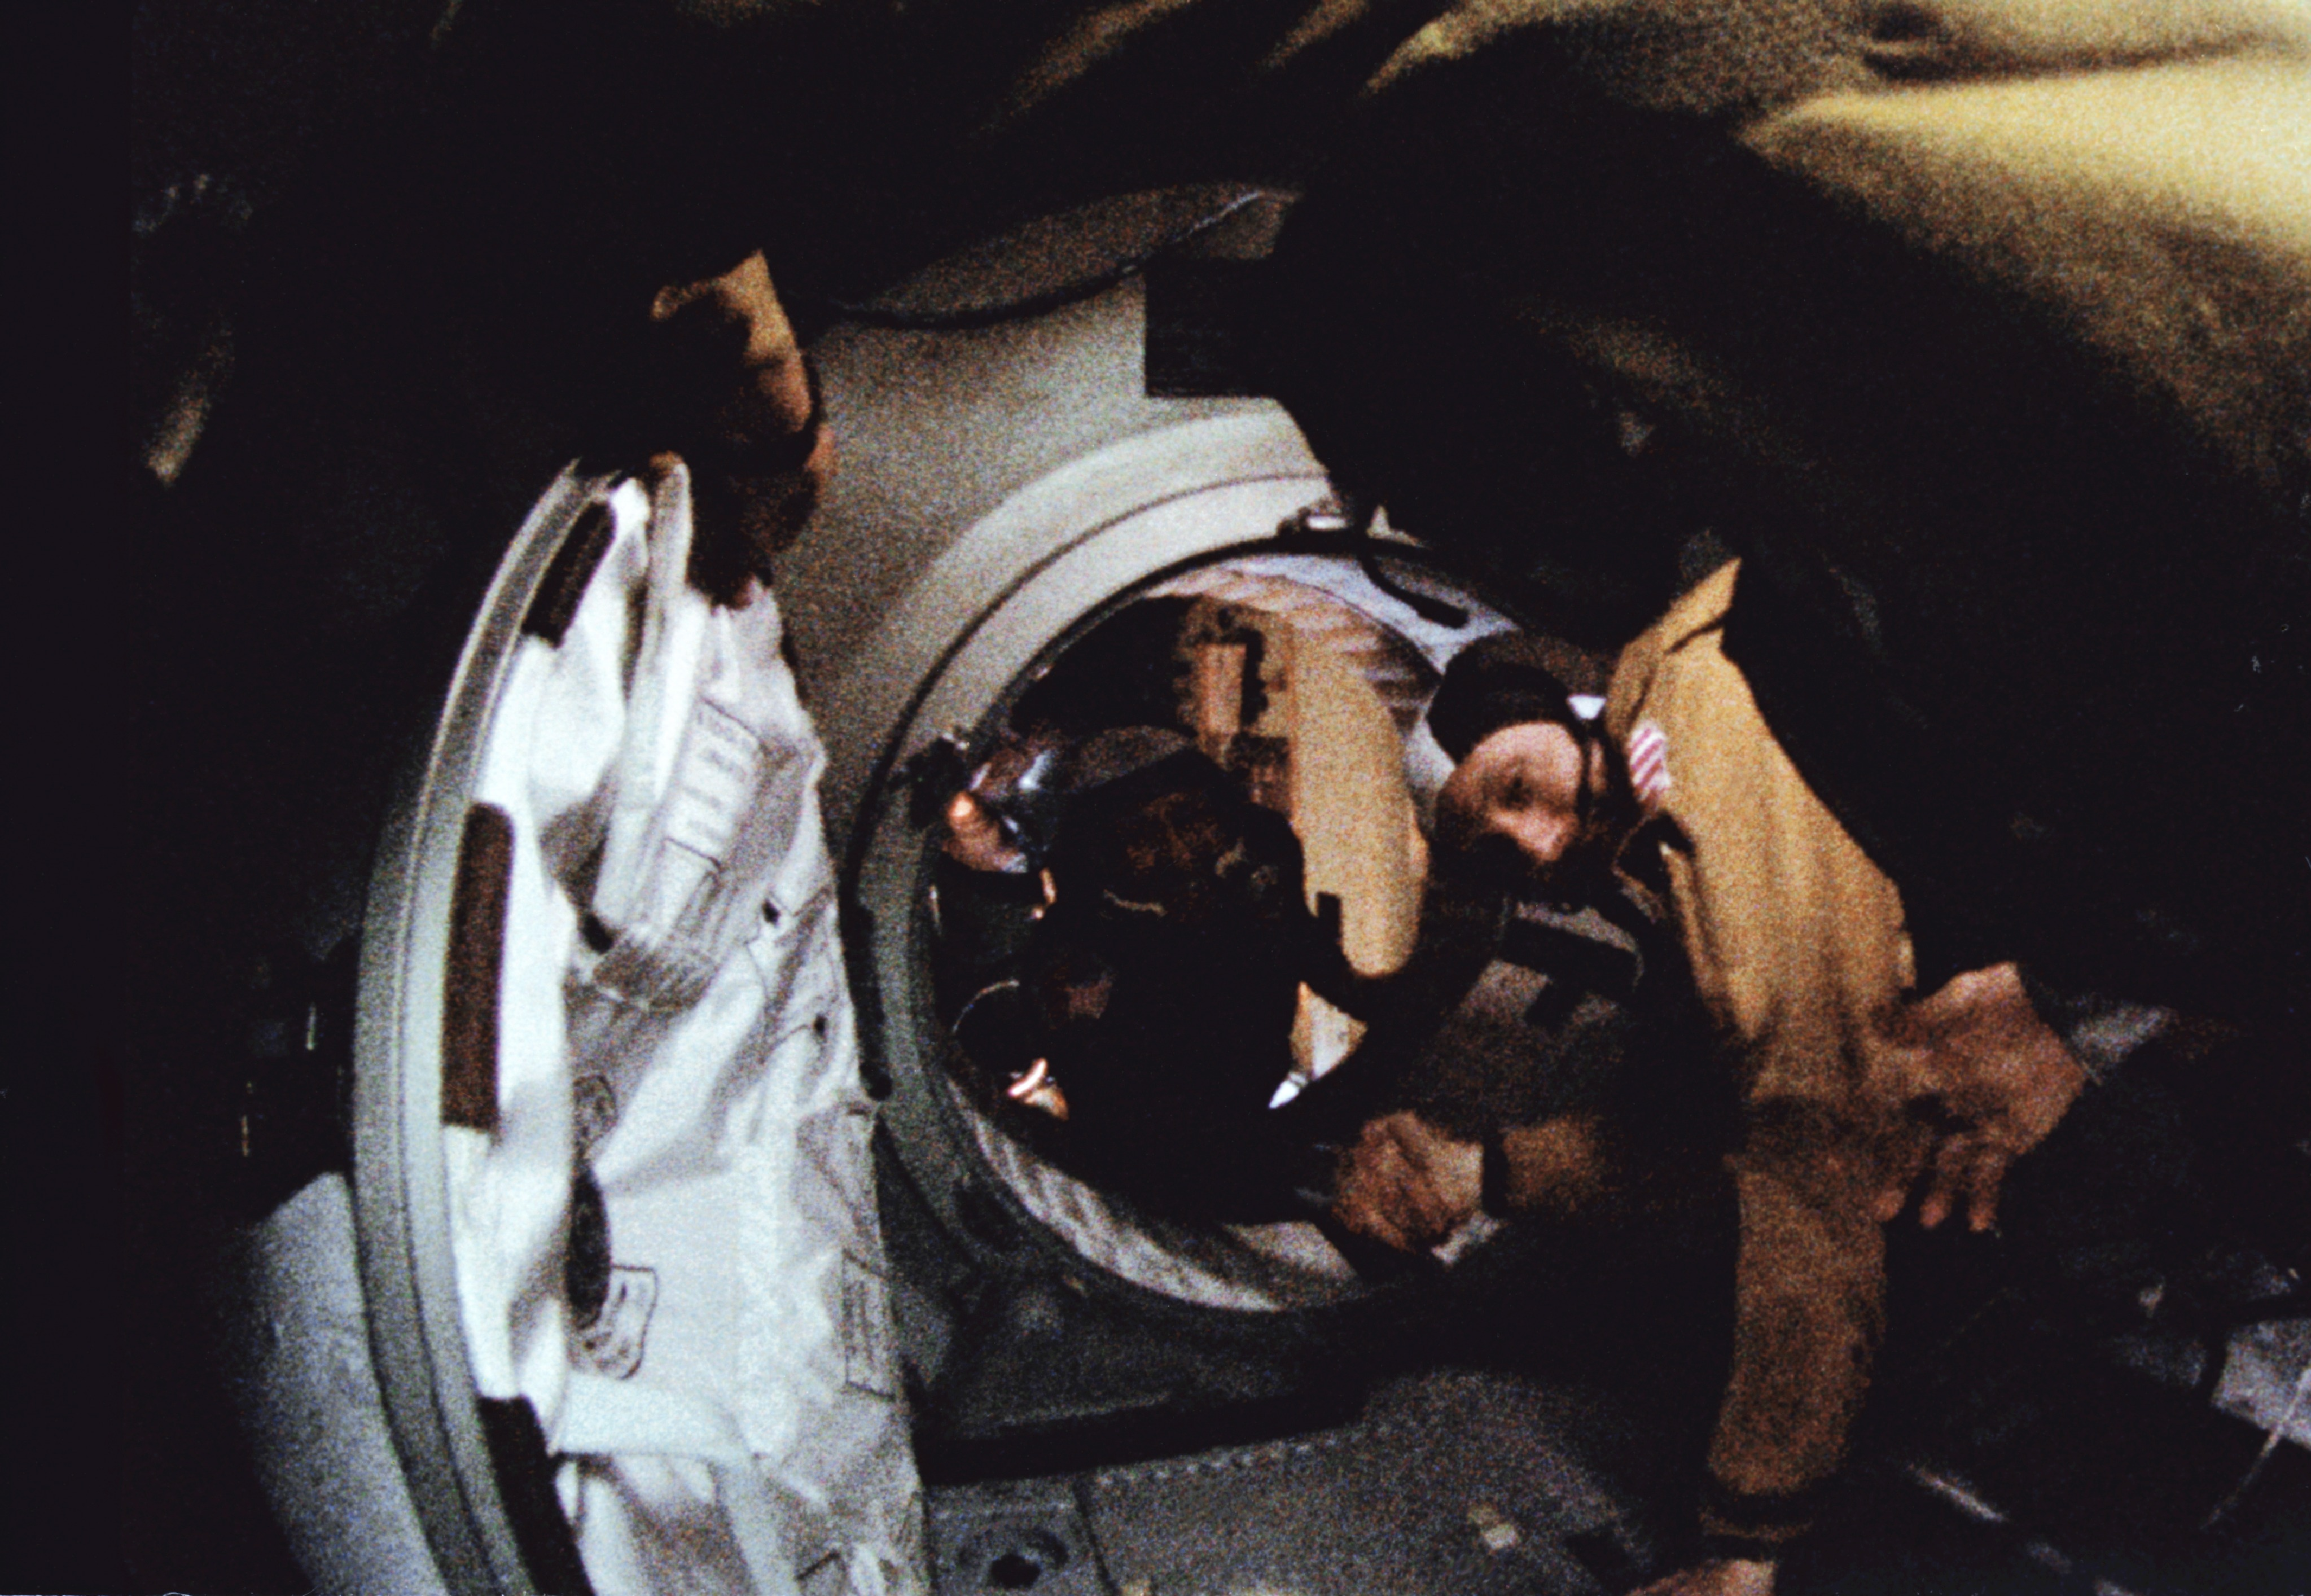
\includegraphics[width=0.88\linewidth,height=0.58\textheight,keepaspectratio]{figures/ch06_iss.jpg}
\caption{Apollo-Soyuz handshake in space - beginning of post-race cooperation.}
\label{fig:ch_apollo_soyuz_handshake_in_space_}
\end{figure}

\bigskip
\begin{otherlanguage}{hebrew}
\subsection*{סיכום הפרק}

פרק זה מסכם את המורשת: סיום עידן אפולו והמעבר מתחרות לשיתוף פעולה בין-לאומי - מאפולו-סויוז ועד תחנת החלל הבין-לאומית.

\end{otherlanguage}

\clearpage
